\documentclass[12pt,a4paper]{article}
% 如果需要中文支持，推荐使用xeCJK + 字体设置
% \usepackage{xeCJK}
% \setCJKmainfont{SimSun}  % 示例：宋体，可根据系统字体情况更换
\usepackage{ctex}
\setlength{\parindent}{2em}
\setlength{\parskip}{0pt} % 确保段落之间没有额外的空行间距


\usepackage{amsmath}      % 数学公式（如有需要）
\usepackage{graphicx}     % 插图
\usepackage{geometry}     % 调整页边距
\usepackage{fancyhdr}     % 自定义页眉页脚
\usepackage{indentfirst}  % 中文首行缩进
\usepackage{calc}         % 允许做长度运算(测量文字宽度等)
\usepackage{titlesec}
\usepackage{booktabs} % 解决 \midrule 和 \bottomrule 报错
\usepackage{enumitem} % 支持自定义列表格式
\usepackage{float}    % 支持强制浮动位置
\usepackage{siunitx}
\usepackage{wrapfig}

% 设置 \section 级标题为：加粗、大字号（如 \Large）
\titleformat{\section}
	{\bfseries\large}    % 标题自身的格式
	{\thesection}        % 标题编号的显示方式
	{1em}                % 编号与标题文字之间的间距
	{}                   % 在标题文字前后可插入额外代码，此处为空
	
% 设置 \subsection 级标题为：加粗、中等字号（如 \normalsize）
\titleformat{\subsection}
	{\bfseries\normalsize}
	{\thesubsection}
	{1em}
{}

% 页面设置（可根据需要微调）
\geometry{
	left=2cm,
	right=2cm,
	top=1cm,
	bottom=1.5cm
}

% 不需要过大的行距，使用较接近单倍行距的设置
\renewcommand{\baselinestretch}{1.2}

% 仅在页脚居中显示页码，页眉保持为空
\pagestyle{fancy}
\fancyhf{}  % 清空默认的页眉页脚
\fancyfoot[C]{\thepage}
\renewcommand{\headrulewidth}{0pt}
\renewcommand{\footrulewidth}{0pt}

% 首行缩进2字符(中文习惯)
% \setlength{\parindent}{0pt}
\setlength{\leftskip}{2em}
\setlength{\parindent}{2em}

\begin{document}
	%-------------------------------------------------------
	% 1 并排两个minipage：左标题、右校徽
	%   - 0.65\textwidth + 0.35\textwidth = \textwidth
	%   - 如果校徽过大或过小，可改宽度，如 0.25\textwidth、0.3\textwidth 等
	%   - 如果想让标题更大，可将 \Huge 改成 \huge 或 \LARGE
	%-------------------------------------------------------
	\noindent
	\hspace{-2em}
	\begin{minipage}[c]{0.65\textwidth}
		\raggedright
		{\fontsize{35pt}{55pt}\selectfont 物理实验报告}
	\end{minipage}
	\begin{minipage}[c]{0.35\textwidth}
		\raggedleft
		% 强制把校徽拉大到 0.35\textwidth 宽度 (高度自动匹配)
		% 若想指定高度,可用 "height=3cm" 等. 二选一即可.
		
\includegraphics[width=\linewidth, trim={20cm 20cm 20cm 20cm}, clip]{university_logo.png}
	\end{minipage}

	\vspace{-1em}
	

	%下方画两条分割线，并在两线之间写学号、姓名、日期、时间
	
	\hrule
	\vspace{0.6em}
	\noindent
	\begin{tabular}{l l l l}
    学号：12411434 & 姓名：{郑宇轩} &
    日期：2025.11.07 & 时间：周五下午
	\end{tabular}
	\vspace{0.4em}
	\par
	\hrule

	
	\section*{\textbf{一. 实验名称：直线运动规律的研究}}
	
	\section*{\textbf{二. 实验目的}}
	\begin{enumerate}
		\item 利用气垫技术测定物体的“瞬时”速度，加速度以及当地的重力加速度；
		\item 利用气垫技术研究一维碰撞的三种情况，验证动量守恒和动能守恒定律；
		\item 定量研究一维碰撞中的动量损失和动能损失。
	\end{enumerate}

	\section*{\textbf{{三. 实验原理}}}

	\begin{enumerate}

	\item \textbf{平均速度和瞬时速度的测量}
	
	作直线运动的物体在 $\Delta t$ 时间内的位移为 $\Delta s$, 则物体在 $\Delta t$ 时间内的平均速度为	$v = \frac{\Delta s}{\Delta t}$；当 $\Delta t \to 0$ 时, 平均速度趋近于一个极限值, 即物体在该点的瞬时速度. 但实验上直接测量某点的瞬时速度是很困难的, 一般在一定误差范围内（小于5\%）, 用极短的 $\Delta t$ 内的平均速度代替瞬时速度.

	\item \textbf{匀变速直线运动}
	
	在一个平斜面上，设有一小滑块在恒定力的作用下做匀加速直线运动。设小滑块初速度为 \( v_0 \)、加速度为 \( a \)、运动时间为 \( t \) 和位移为 \( s \)，则运动学关系可描述为：
			\[v = v_0 + at,\quad s = v_0 t + \frac{1}{2}at^2 \quad \Rightarrow \quad v^2 = v_0^2 + 2as\]
			当小滑块从不同的位置开始滑动（对于起始时刻可视为 \( v_0 = 0 \)），在同一位置测量其速度时，若绘制 \( v^2 \) 与 \( s \) 的关系图，将得到一条直线，其斜率为 \( 2a \)。

		\item \textbf{重力加速度的测定}
		
		\begin {figure}[H]
			\centering	
			
\includegraphics[width=0.4\textwidth]{1.jpg}
			\caption{实验装置示意图}
			\label{fig:fig1}
		\end{figure}
			如图1所示，记 \( h \) 为斜块的高度，\( L \) 为斜面的长度，块沿斜面下滑的加速度为：
			\[a = g\sin\theta = g\frac{h}{L} \quad \Rightarrow \quad g = \frac{aL}{h}\]

		\item \textbf{碰撞过程中守恒定律的研究}
		
			如果一个力学系统所受合外力为零或在某方向上的合外力为零，则该力学系统总动量守恒或在某方向上守恒，即：$\sum m_i v_i = \text{constant}$
			对于三种碰撞情形，动量和动能守恒情形如下：
			\begin{itemize}
    			\item[(a)] 完全弹性碰撞:动量守恒，能量守恒
    			\item[(b)] 完全非弹性碰撞:动量守恒，动能不守恒
    			\item[(c)] 一般非弹性碰撞:动量守恒，动能不守恒
			\end{itemize}


	
	\end{enumerate}
	
	\section*{\textbf{{四. 实验仪器}}}
	气垫导轨实验仪器、电子计时器、滑块、天平

	\section*{\textbf{{五. 实验内容}}}

	\begin{enumerate}
		\item \textbf{匀变速运动中速度与加速度的测量}
		
			\begin{enumerate}
				\item 先将气垫导轨调平（动平调法：两光电门间距离50.00cm以上，轻轻推动大滑块，使其通过第一个光电门的时间 $t_1 > 80\,\text{ms}$，并且通过第二个光电门的时间 $t_2$ 满足 $t_1 - 5 < t_2 < t_1 + 5$），然后在一端单脚螺丝下置一滑块，使导轨成一斜面。
				\item 在大滑块上装上 U 型挡光片，调节光电门，打开计时装置，使用“计时2”测试。
				\item 使大滑块分别从距离光电门 $S = 20.00\,\text{cm}, 30.00\,\text{cm}, 40.00\,\text{cm}, 50.00\,\text{cm}, 60.00\,\text{cm}$ 处自然下滑，进行初速度为零的匀加速运动，记下挡光时间 $\Delta t$，每个 $S$ 情况下重复测量三次。
				\item 测量 U 型挡光片有效长度 $\Delta s$（测3次）、斜面高度 $h$（测3次）及斜面长度 $L$（测1次）。
				\item 根据 U 型挡光片有效长度 $\Delta s$ 和挡光时间 $\Delta t$，计算出速度 $v$；根据公式 $v^2 = 2as$ 用 Origin 软件进行直线拟合，求出加速度 $a$，并计算重力加速度 $g$。深圳市参考重力加速度 $g_0 \approx 9.7883\,\text{m/s}^2$）。
			\end{enumerate}
		\item \textbf{研究三种碰撞状态下的守恒定律}	
			\begin{enumerate}
				\item 撤掉气垫导轨的垫块，按计时器上的“功能”键，选择“碰撞”档位。
				\item 取大小两滑块A、B，将两滑块分别装上弹簧钢圈，用物理天平称量此时滑块A、B的质量，分别记为 $m_1$ 和 $m_2$，且保证 $m_1 > m_2$。打开气泵，将小滑块B置于两光电门之间（两光电门的距离为30.00--40.00 cm），使其静止。用 $m_1$ 碰撞 $m_2$，分别记录 $m_1$ 通过第一个光电门的时间 $\Delta t_{11}$ 和经过第二个光电门的时间 $\Delta t_{12}$，以及 $m_2$ 通过第二个光电门的时间 $\Delta t_{21}$，重复三次，记录所测数据。
				\item 分别在两滑块上换上尼龙搭扣，重复上述测量步骤。
				\item 分别在两滑块上换上金属碰撞器，重复上述测量步骤。
				\item 分别计算每种碰撞下动量的变化、动能的变化，计算动量损失率 $\Delta p/p$ 和动能失率 $\Delta E/E$，并根据计算数据得出相应的实验结论。
			\end{enumerate}

	\end{enumerate}
	
	\section*{\textbf{{六. 数据记录}}}
	
	原始测量数据见附表 1。

	\section*{\textbf{{七. 数据处理}}}

	\begin{enumerate}


	\item \textbf{匀变速运动中速度与加速度的测量}
	
		$\Delta s = \dfrac{\Delta s_1 + \Delta s_2 + \Delta s_3}{3} = \dfrac{1.00 + 1.00 + 1.00}{3} = 1.00\mathrm{cm}$

		$h = \dfrac{h_1 + h_2 + h_3}{3} = \dfrac{0.94 + 0.93 + 0.95}{3} = 0.94\mathrm{cm}$

		$L = \dfrac{87.35 + 84.45}2 = 85.9\mathrm{cm}$
	
		根据$v=\frac{\Delta s}{t}$计算得到$v^2$，如下图所示：
		
			\begin{figure}[H]
				\centering
				
\includegraphics[width=0.75\textwidth]{2.jpg}
				\caption{$v^2$数据表}
				\label{fig:fig2}
	  		\end{figure}

		作出$v^2—s$的直线拟合，如下图所示：
		  	\begin{figure}[H]
				\centering
				
\includegraphics[width=0.75\textwidth]{3.jpg}
				\caption{$v^2 - s$ 直线拟合图}
				\label{fig:fig3}
	  		\end{figure}
			线性拟合方程为 $v^2=0.2136x+0.0037 \quad R^2=0.99998$。
			
			则 $a = 0.1068\mathrm{m/s^2}$，$g = \dfrac{aL}{h} = \dfrac{0.1068 \times 85.9}{0.94} = 9.7597\,\text{m/s}^2$；
			
			相对误差为$\epsilon=\dfrac{\lvert g_{0}-g \rvert}{g_{0}}\times 100\% = \dfrac{|9.7597 - 9.7883|}{9.7883} =  0.29\%$
			
	\item \textbf{研究三种碰撞状态下的守恒定律}

		\begin{itemize}
			
			\item \textbf{完全弹性碰撞}
			
				$m_1 = 204.04\mathrm{g},\ m_2 = 115.57\mathrm{g}$

				由 $p = mv, E_k = \dfrac{1}2 mv^2$以及 $v = \dfrac{\Delta s}{t}$，可得到碰撞前后的动量和动能，如下图所示：

				\begin{figure}[H]
					\centering
					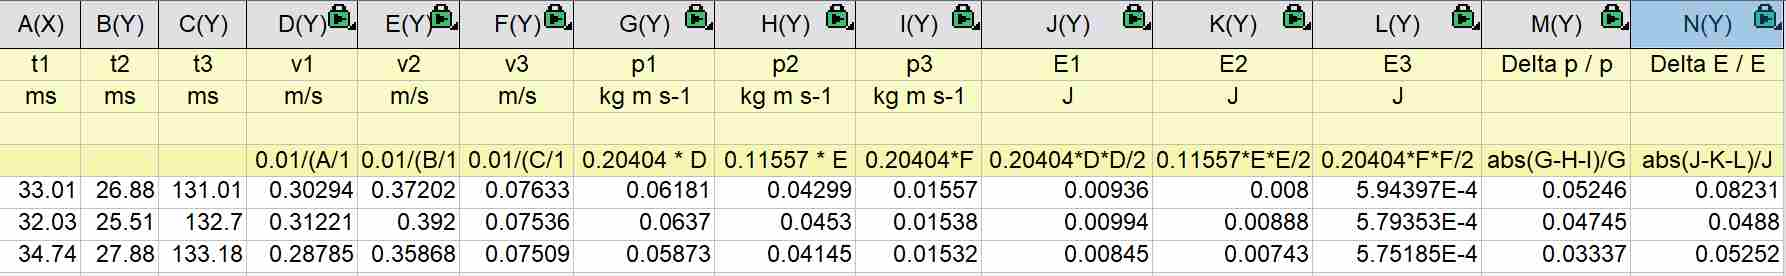
\includegraphics[width=1\textwidth]{4.jpg}
					\caption{完全弹性碰撞动量动能表}
					\label{fig:fig4}
				\end{figure}
				
				$\eta_{p_1} = \dfrac{\Delta p_1}{p_1} = 5.246\%$，$\eta_{p_2} = \dfrac{\Delta p_2}{p_2} = 4.745\%$，$\eta_{p_3} = \dfrac{\Delta p_3}{p_3} = 3.337\%$

				$\eta_{E_1} = \dfrac{\Delta E_1}{E_1} = 8.231\%$，$\eta_{E_2} = \dfrac{\Delta E_2}{E_2} = 4.880\%$，$\eta_{E_3} = \dfrac{\Delta E_3}{E_3} = 5.252\%$

				在误差允许范围内：\textbf{动量守恒，动能守恒}。

			\item \textbf{完全非弹性碰撞}
			
			$m_1 = 213.93\mathrm{g},\ m_2 = 115.15\mathrm{g}$

			由 $p = mv, E_k = \dfrac{1}2 mv^2$以及 $v = \dfrac{\Delta s}{t}$，可得到碰撞前后的动量和动能，如下图所示：
				\begin{figure}[H]
					\centering
					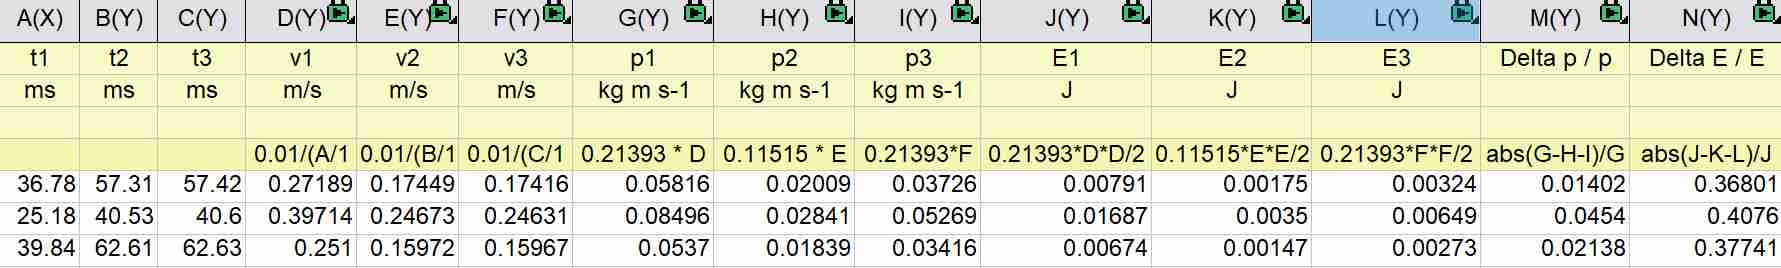
\includegraphics[width=1\textwidth]{5.jpg}
					\caption{完全非弹性碰撞动量动能表}
					\label{fig:fig5}
				\end{figure}
				则 
				$\eta_{p_1} = \dfrac{\Delta p_1}{p_1} = 1.402\%$，$\eta_{p_2} = \dfrac{\Delta p_2}{p_2} = 4.540\%$，$\eta_{p_3} = \dfrac{\Delta p_3}{p_3} = 2.138\%$

				$\eta_{E_1} = \dfrac{\Delta E_1}{E_1} = 36.801\%$，$\eta_{E_2} = \dfrac{\Delta E_2}{E_2} = 40.760\%$，$\eta_{E_3} = \dfrac{\Delta E_3}{E_3} = 37.741\%$

				
				在误差允许范围内，\textbf{动量守恒，动能不守恒}。

			\item \textbf{非完全弹性碰撞}

			$m_1 = 211.65\mathrm{g},\ m_2 = 112.79\mathrm{g}$

			由 $p = mv, E_k = \dfrac{1}2 mv^2$以及 $v = \dfrac{\Delta s}{t}$，可得到碰撞前后的动量和动能，如下图所示：
				\begin{figure}[H]
					\centering
					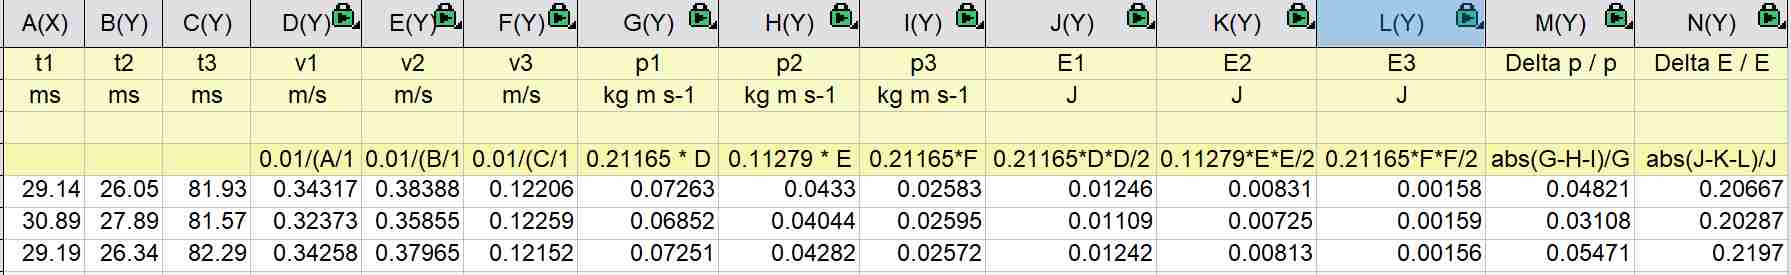
\includegraphics[width=1\textwidth]{6.jpg}
					\caption{非完全弹性碰撞动量动能表}
					\label{fig:fig6}
				\end{figure}
				则 
				$\eta_{p_1} = \dfrac{\Delta p_1}{p_1} = 4.821\%$，$\eta_{p_2} = \dfrac{\Delta p_2}{p_2} = 3.108\%$，$\eta_{p_3} = \dfrac{\Delta p_3}{p_3} = 5.471\%$

				$\eta_{E_1} = \dfrac{\Delta E_1}{E_1} = 20.667\%$，$\eta_{E_2} = \dfrac{\Delta E_2}{E_2} = 20.287\%$，$\eta_{E_3} = \dfrac{\Delta E_3}{E_3} = 21.970\%$
				
				在误差允许范围内，\textbf{动量守恒，动能不守恒}。
			\end{itemize}

	\end{enumerate}
	
	\section*{\textbf{八. 误差分析}}

	\begin{enumerate}
		\item 气垫导轨未完全平衡摩擦力等阻力；
		\item 各次实验下滑位置和初速度不固定，且无法保证初速度为 0。
	\end{enumerate}

	\section*{\textbf{{九. 问题思考}}}

	\begin{enumerate}
			\item 气垫导轨调水平的判断标准是什么？\\
			气垫导轨调水平的主要判断标准是观察放置其上的滑块在沿同一方向移动时能否做匀速直线运动。若滑块在被轻推后能保持匀速运动，则表明导轨已基本水平。
		
			\item 如何减小气垫导轨气流阻力对实验的影响？\\
			确保足够的气压和气流量以形成稳定的气垫；保持导轨和滑块表面的清洁光滑；尽量缩短实验时间和滑块的运动距离。
		
			\item 碰撞前后系统总动量不相等（可能出现碰撞后动量减小或增加），试分析其原因。\\
			实验中存在外力作用，如未被完全平衡的摩擦力和空气阻力等；实验操作产生的误差也可能导致测得动量不守恒。
		\end{enumerate}


	
	\section*{\textbf{{十. 实验结论}}}

	\begin{enumerate}
		\item  实测重力加速度$g = 9.7597 \,\text{m/s}^2$,相对误差$\epsilon = 0.29\%$

		\item  对于不同碰撞状态：
		\begin{itemize}
			\item \textbf{完全弹性碰撞}\\
				动量损失率 $\eta_{p_1}=5.246\%>5\%,\eta_{p_2}=4.745\%<5\%,\eta_{p_3}=3.337\%<5\%$

				动能损失率 $\eta_{E_1}=8.231\%>5\%,\eta_{E_2}=4.880\%<5\%,\eta_{E_3}=5.252\%>5\%$

				在误差允许范围内，动量守恒，动能守恒。
			\item \textbf{完全非弹性碰撞}\\
				动量损失率 $\eta_{p_1}=1.402\%<5\%,\eta_{p_2}=4.540\%<5\%,\eta_{p_3}=2.138\%<5\%$

				动能损失率 $\eta_{E_1}=36.801\%>5\%,\eta_{E_2}=40.760\%>5\%,\eta_{E_3}=37.741\%>5\%$

				在误差允许范围内，动量守恒，动能不守恒。
			\item \textbf{非完全弹性碰撞}\\
				动量损失率 $\eta_{p_1}=4.821\%<5\%,\eta_{p_2}=3.108\%<5\%,\eta_{p_3}=5.471\%>5\%$

				动能损失率 $\eta_{E_1}=20.667\%>5\%,\eta_{E_2}=20.287\%>5\%,\eta_{E_3}=21.970\%>5\%$

				在误差允许范围内，动量守恒，动能不守恒。

		\end{itemize}
	\end{enumerate}

\end{document}